\documentclass[tikz]{standalone}
\usepackage{tikz}
\usepackage{verbatim}
\usetikzlibrary{shapes,arrows,fit,calc,positioning}


\begin{document}

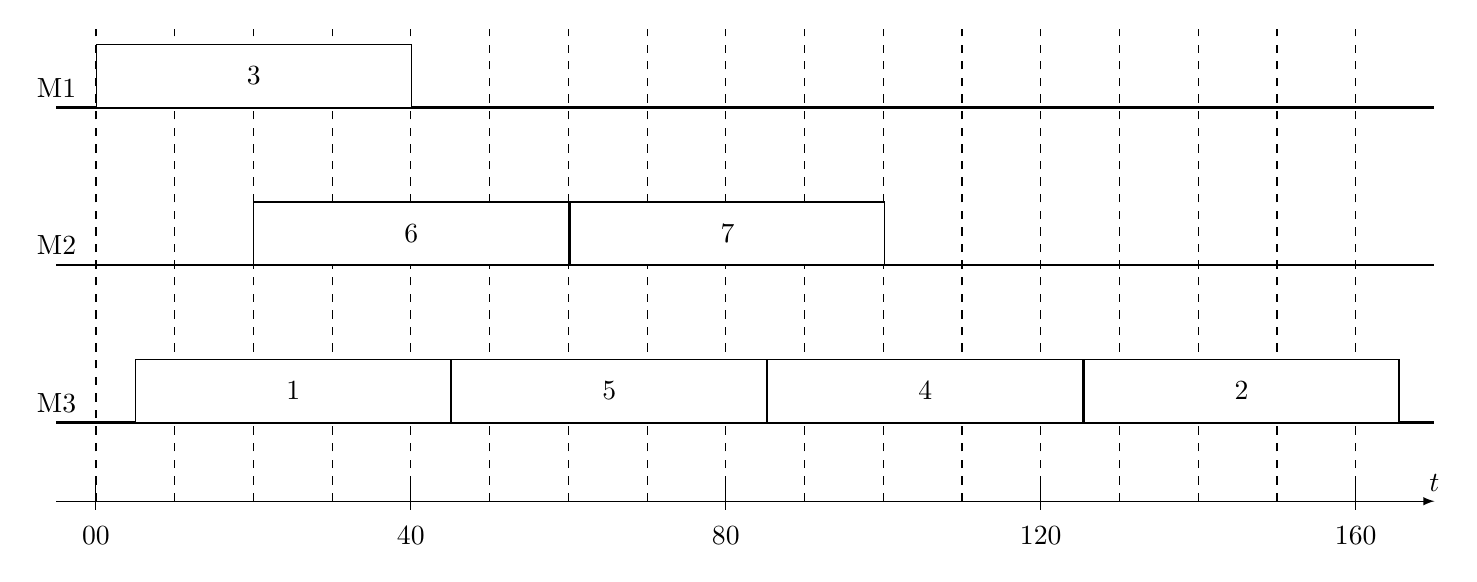
\begin{tikzpicture}[xscale=1,transform shape]

\draw [-latex](-0.5,0) coordinate(dd)-- (0,0) coordinate (O1) -- (17,0)coordinate(ff) node[above]{$t$};
\draw [dashed,thick] (O1) -- (0,1) coordinate(M3) -- (0,3) coordinate(M2) -- (0,5) coordinate(M1) -- ++(0,1)coordinate(ff2);

\foreach \nn in{M3,M2,M1}{
\draw [thick] (dd|-\nn) node[above]{\nn}-- (\nn-|ff);
}

\foreach \xx in{1,2,...,16}{
\draw[dashed] (\xx,0) -- (\xx,0|- ff2);
}

\foreach \xx in{0,4,8,...,16}{
\draw[dashed] (\xx,0.2) -- (\xx,-0.2) node[below]{\xx 0};
}

\begin{scope}[shift={(M1)}]
\node[ above right=0.4cm and 0cm of M1,right,draw, minimum width=4cm,minimum height=0.8cm,fill=white](n3a) {$3$};
\end{scope}

\begin{scope}[shift={(M2)}]
\coordinate(O2) at (2,0);
\node[ above right=0.4cm and 0cm of O2,right,draw, minimum width=4cm,minimum height=0.8cm,fill=white](n4a) {$6$};
\node[right=0cm of n4a,right,draw, minimum width=4cm,minimum height=0.8cm,fill=white](n3b) {$7$};
\end{scope}

\begin{scope}[shift={(M3)}]
\coordinate(O3) at (0.5,0);
\node[ above right=0.4cm and 0cm of O3,right,draw, minimum width=4cm,minimum height=0.8cm,fill=white](n1) {$1$};
\node[right=0cm of n1,right,draw, minimum width=4cm,minimum height=0.8cm,fill=white](n5) {$5$};
\node[right=0cm of n5,right,draw, minimum width=4cm,minimum height=0.8cm,fill=white](n4b) {$4$};
\node[right=0cm of n4b,right,draw, minimum width=4cm,minimum height=0.8cm,fill=white](n3c) {$2$};
\end{scope}

\end{tikzpicture}

\end{document}